\section{Obtención de los parámetros dinámicos del robot}

Al obtener las matrices del modelo dinámico, ya seremos capaces de predecir el comportamiento de nuestro robot en la realidad; 
una vez que determinemos las incertidumbres paramétricas que se especificaron al inicio del apartado anterior.
Osea se, que aunque tengamos estructuradas las matrices, no seremos capaces de determinar el comportamiento
del robot, ya que, tenemos un compendio de incertidumbres, que deberán ser determinadas numéricamente.\\


Por tanto, este apartado esclarecerá como resolver las incertidumbres paramétricas presentes, mediante
técnicas de regresión lineal y la realización de experimentos sobre el propio robot, para determinar las siguientes
incógnitas definidas en Matlab como variables simbólicas:

\begin{itemize}
	\item HABLAR UN POCO DE LA NECESIDAD DE ESTIMAR LOS PARAMETROS DE NEWTON EULER

\end{itemize}

\begin{center}
		$ I_{11} =
	\begin{bmatrix}
	I_{11xx} & I_{11xy} & I_{11xz}\\
	I_{11yx} & I_{11yy} & I_{11zz}\\
	I_{11zx} & I_{11zy} & I_{11zz}
	\end{bmatrix} $
	\vspace{0.75cm}
	$ I_{22} =
	\begin{bmatrix}
	I_{22xx} & I_{22xy} & I_{22xz}\\
	I_{22yx} & I_{22yy} & I_{22zz}\\
	I_{22zx} & I_{22zy} & I_{22zz}
	\end{bmatrix}$
	\vspace{0.75cm}
	$ I_{33} =
	\begin{bmatrix}
	I_{33xx} & I_{33xy} & I_{33xz}\\
	I_{33yx} & I_{33yy} & I_{33zz}\\
	I_{33zx} & I_{33zy} & I_{33zz}
	\end{bmatrix}$
	\vspace{0.75cm}
	$ Jm =
	\begin{bmatrix}
	Jm_{1} \\
	Jm_{2} \\
	Jm_{3}
	\end{bmatrix}$
	\vspace{0.75cm}
	$ Bm =
	\begin{bmatrix}
	Bm_{1} \\
	Bm_{2} \\
	Bm_{3}
	\end{bmatrix}$
	
TERMINAR DE METER MATRICES LOCO
\end{center}

	\subsection{Estimación de parámetros dinámicos}
		Primero reestructuraremos nuestro modelo dinámico en dos matrices en las que, por un lado,
		se agrupen las incertidumbres dinámicas en una matriz \textit{theta}, y por otro, el resto de nuestro modelo 
		dinámico en una matriz \textit{phi} que dependerá de las variables articulares del robot.
	
		
		\begin{equation}
			\tau=M(q)\ddot{q}+V(q,\dot{q})+G(q) \hspace{1.25cm}  \rightarrow \hspace{1.25cm} \tau=\phi(x) \hspace{0.25cm} \theta
			\end{equation}
			
	
	
	Agrupando en \textit{theta} el conjunto de las incertidumbres obtenemos el vector de términos resultante.


	\begin{equation}
		\theta=
			\begin{pmatrix}
				I_{11xx} \\
				I_{11yy}\\
				I_{11zz}\\
				Jm_{1} \\
				Bm_{1} \\
				I_{22xx} \\
				I_{22yy}\\
				I_{22zz}\\
				Jm_{2} \\
				Bm_{2} \\
				I_{33xx} \\
				I_{33yy}\\
				I_{33zz}\\
				Jm_{3} \\
				Bm_{3} \\
				m_{1}s_{11z}^{2} \\
				m_{1}s_{11z} \\
				m_{1}\\
				m_{2}s_{22x}^{2} \\
				m_{2}s_{22x} \\
				m_{2}\\
				m_{3}s_{33x}^{2} \\
				m_{3}s_{33x} \\
				m_{3}
				\end{pmatrix}
		\end{equation}

		Si usamos esta vector \textit{theta} como base para re-ordenar nuestro modelo dinámico, vemos, en la matriz resultante \textit{phi}, 
		que existen columnas repletas de ceros, o relaciones lineales entre las columnas, por lo que, se deberán
		agrupar aquellos términos que no sean linealmente independientes y eliminar los términos asociados
		a las columnas de ceros, ya que significará que no tienen relevancia en nuestro modelo dinámico.\\

		Para poder agrupar los parámetros linealmente independientes, nos apoyaremos en Matlab para poder gestionar
		estas matrices de gran tamaño.\\
		Se deben dar valores aleatorios a los parámetros articulares que aparecerán en la matriz \textit{phi}, y sustituir estos 
		valores dentro de la matriz; posteriormente se elegirán otros valores para las variables articulares,  y se concatenarán
		con la matriz anterior. Este proceso se repetirá hasta obtener una matriz concatenada de iguales dimensiones de ancho y largo.\\
		
		Obteniendo esta matriz cuadrada podremos ejecutar el comando \textit{rref()} que nos devolverá las relaciones entre las columnas de la matriz
		\textit{phi}, y que serán las mismas relaciones que dentro de las filas del vector de incertidumbres \textit{theta}.\\
		
		\begin{equation}
			\theta=
				\begin{pmatrix}
					  m_{1}s_{11z}^{2} + m_{2}s_{22x}^{2} + m_{3}s_{33x}^{2} + I_{11yy} + I_{22yy} + I{33yy} + R_{1}^{2}Jm_1 - m_2 - 1.64m_3 \\
					  Bm_{1}  \\
					  -m_{2}s_{22x}^{2} + I_{22xx} - I_{22yy} + m_{2} + m_{3} \\
					  m_{2}s_{22x}^{2} + I_{22zz} + R_{2}^{2}Jm_{2} - m_{2} - m_{3}  \\
					  Bm_{2} \\
					  - m_{3}s_{33x}^{2} + I_{33xx} - I_{33yy} + 0.64m_{3} \\
					  m_{3}s_{33x}^{2} + I_{33zz} - 0.64m_{3}  \\
					  Jm_{3}  \\
					  Bm_{3}  \\
					  -m_{2} -m_{3} + m_{2}s_{22x}  \\
					  m_{3}s_{33x} - 0.8m_{3}
				\end{pmatrix}
			\end{equation}



			\[
\gamma=
\begin{pmatrix}
\ddot{q_1} & R_{1}^{2}\dot{q_1} & \gamma_{1,3} & 0 & 0  & \gamma_{1,6} & 0 & 0 & 0 & \gamma_{1,10} & \gamma_{1,11} \\
0 & 0 & \gamma_{2,3} & \ddot{q_2} & R_{2}^{2}\dot{q_2} & \gamma_{2,6} & \ddot{q_2} + \ddot{q_3} & 0 & 0 & \gamma_{2,10} & \gamma_{2,11} \\
0 & 0 & 0 & 0 & 0 & \gamma_{3,6} & \ddot{q_2} + \ddot{q_3} & R_{3}^{2}\ddot{q_3} & R_{3}^{2}\ddot{q_3} & 0 & \gamma_{3,11} \\
\end{pmatrix} \] \vspace{0.3cm}

\begin{itemize}
\item $\gamma_{1,3}=\frac{\ddot{q_1}}{2} - \frac{\ddot{q_1}cos(2q_2)}{2} + \dot{q_1}\dot{q_2}sin(2q_2) $ \\ \vspace{0.2cm}
\item $\gamma_{1,6}=\frac{\ddot{q_1}}{2} - \frac{\ddot{q_1}cos(2q_2 + 2q_3)}{2} +\dot{q_1}\dot{q_2}sin(2q_2 + 2q_3) + \dot{q_1}\dot{q_3}sin(2q_2 + 2q_3) $\\ \vspace{0.2cm}
\item $\gamma_{1,10}=-L_{2}(\ddot{q_1} + \ddot{q_1}cos(2q_2) - 2\dot{q_1}\dot{q_2}sin(2q_2))$ \\ \vspace{0.2cm}
\item  $\gamma_{1,11}=2L_3\dot{q_1}\dot{q_2}sin(2q_2 + 2q_3) - L2\ddot{q_1}cos(2q_2 + q_3) - L_{3}\ddot{q_1}cos(2q_2 + 2q_3) - L2\ddot{q_1}cos(q_3) - L_{3}\ddot{q_1}$ + \\ \vspace{0.1cm}
	$+2L_{3}\dot{q_1}\dot{q_3}sin(2q_2 + 2q_3) + L_{2}\dot{q_1}\dot{q_3}sin(q_3) + 2L_{2}\dot{q_1}\dot{q_2}sin(2q_2 + q_3) + L_{2}\dot{q_1}\dot{q_3}sin(2q_2 + q_3)$ \\ \vspace{0.2cm}
\item $\gamma_{2,3}=-\frac{\dot{q_1}^{2}sin(2q_2)}{2} $\\ \vspace{0.2cm}
\item $\gamma_{2,6}=-\frac{\dot{q_1}^{2}sin(2q_2 + 2q_3)}{2} $\\ \vspace{0.2cm}
\item $\gamma_{2,10}= - L_{2}sin(2q_2)\dot{q_1}^{2} - 2L_{2}\ddot{q_2} - g*cos(q_2)$ \\ \vspace{0.2cm}
\item $\gamma_{2,11}=  L_{2}{q_3}^{2}sin(q_3) - 2L3\ddot{q_3} - g*cos(q_2 + q_3) - 2L_{3}\ddot{q_2} - L_{2}\dot{q_1}^{2}sin(2q_2 + q_3) - $\\ \vspace{0.1cm}
	$- L_{3}\dot{q_1}^{2}sin(2q_2 + 2q_3) - 2L_2\ddot{q_2}cos(q_3) - L_{2}\ddot{q_3}cos(q_3) + 2L_{2}\dot{q_2}\dot{q_3}sin(q_3) $\\ \vspace{0.2cm}
\item $\gamma_{3,6}=-\frac{\dot{q_1}^{2}sin(2q_2 + 2q_3)}{2} $\\ \vspace{0.2cm}
\item $\gamma_{3,11}=- 2L_{3}\ddot{q_2} - 2L_3\ddot{q_3} - g*cos(q_2 + q_3) - \frac{L_{2}\dot{q_1}^{2}sin(q_3)}{2} - L_2\dot{q_2}^{2}sin(q_3) - $\\ \vspace{0.1cm}
$-\frac{L_2\dot{q_1}^{2}sin(2q_2 + q_3)}{2} - L_{3}\dot{q_1}^{2}sin(2q_2 + 2q_3) - L_2\ddot{q_2}cos(q_3) $\\


Para verificar que no se ha cometido errores en este procedimiento basta con multiplicar las dos matrices obtenidas, y restarlo al modelo dinámico
que se obtuvo con el algoritmo de Newton-Euler, ya que, al ser una reorientación de parámetros, este resultado debe ser 0; por lo que 
si este resultado es diferente se debe comprobar el proceso en busca de errores.
\end{itemize}

	\begin{itemize}
	
		\item HABLAR DE COMO SE OBTUVO GAMMA SIM Y TETHA SIM
		\item HABLAR DE LA SIMPLIFICACION A PARAMETROS LI
	


	\end{itemize}
	
	\newpage

	\subsection{Identificación y cálculos estadísticos}

	Una vez que agrupados correctamente los términos linealmente independientes de nuestra estructuradas
	\textit{phi}-\textit{theta}, se procederá a la realización de los experimentos sobre
	el robot en cuestión, y la determinación de estas incertidumbres dinámicas.\\

	Como se explicó en clases, esta identificación se basa en la regresión lineal con la minimización de los 
	errores cuadráticos, para ello, necesitaremos realizar un numero de experimentos mucho mas elevado que el número
	de incertidumbres que tenemos en la matriz \textit{theta} linealmente independiente. Además, se deberá hacer
	un mínimo diseño de los experimentos a los que se va a someter el robot para la búsqueda de estos parámetros.\\

	Sobre los experimentos y la metodología que seguida. Tenemos unos parámetros están fuertemente asociados a determinados
	valores de las variables articulares; se puede ver esta dependencia al analizar el modelo dinámico de Newton-Euler.
	 Ante esto, podemos deducir a priori, que ciertos parámetros estarán mas representados ante ciertas condiciones de funcionamiento; esto será lo que determinara la
	veracidad del experimento, y de donde sacaremos las consignas para el diseño de estos.\\

	\begin{itemize}
		\item Parametros Gravitarios $ \rightarrow $
		\item Parametros Inerciales $ \rightarrow $
		\item Parametros Viscosos $ \rightarrow $
		
	\end{itemize}

	

	



	\begin{itemize}
	
		\item HABLAR DE LOS EXPERIMENTOS DE LOS SENOS
		\item HABLAR DE LA OPTIMIZACION Y ESTIMACION DE LOS PARAMETROS
	\end{itemize}


	\subsection{Parametros y modelos obtenidos}
	A continuación, se mostrarán los parámetros obtenidos para cada configuración del robot, así cómo la covarianza con la que se han obtenido los mismos.\\
	Para evitar repetir siempre los parámetros, se irán definiendo componente a componente, es decir, a continuación se definirá tetha con todos los parámetros y se dirá en cada caso concreto la posición del parámetro obtenido en el vector, el valor de dicho parámetro y la covarianza del mismo. \\

	Además de ello, se obtendrán las ecuaciones dinámicas que definen el comportamiento dinámico de las articulaciones del robot. Para obtener éstas ecuaciones, será necesario multiplicar la matriz $\gamma$ que posteriormente se definirá por la matriz $\theta$ con valores numericos. \\
	Una vez se tengan las ecuaciones dinámicas del robot, al igual que se hizo cuando se aplicó el algoritmo de \textit{Newton-Euler}, se irán derivando las expresiones respecto las posiciones, velocidades y aceleraciones articulares para obtener las matrices de inercias, matriz de terminos de Coirolis y la matriz formada por los términos gravitarios.\\

	Por último, cabe destacar que los modelos con medidas reales se han obtenido a partir de la posición del modelo real cuantizada, es decir, para obtener la velocidad y la aceleración fue necesario la aplicación de filtros no causales y la aplicación de filtros que limpien los ruidos.


La matriz $\gamma$ obtenida que, multiplicada por los valores numéricos de $\theta$, resultarán las ecuaciones dinámicas del robot estudiado, se muestra a continuación:



	\subsubsection{Robot medidas ideales con reductoras}
	Los parametros estimados, es decir, la matriz tetha linealmente independiente de 11 parámetros, obtenida para desarrollar el modelo del robot con medidas ideales con reductoras en los motores será:
	\begin{center}
		\begin{tabular}{| c | c | c |}

			\hline
			Parametro estimado & Valor obtenido & Covarianza obtenida \\
			\hline
			$\theta(1) $ & 15.6322 & 0.0338 \\
			\hline
			$\theta(2) $ & 0.0012 & 0.0218 \\
			\hline
			$\theta(3) $ & 7.389 & 0.0481 \\
			\hline
			$\theta(4) $ & 55.1139 & 0.00081 \\
			\hline
			$\theta(5) $ & 0.00085 & 0.02744 \\
			\hline
			$\theta(6) $ & 2.0841 & 0.047868 \\
			\hline
			$\theta(7) $ & -2.0414 & 0.00623 \\
			\hline
			$\theta(8) $ & 0.051 & 0.00113 \\
			\hline
			$\theta(9) $ & 0.0015 & 0.033 \\
			\hline
			$\theta(10) $ & -6.665 & 0.00054 \\
			\hline
			$\theta(11) $ & -2.222 & 0.00113 \\
			\hline


		\end{tabular}
	\end{center}
Por lo tanto, tras multiplicar $\gamma$ y $\theta$ y derivar respecto a las variables articulares, se definirán las ecuaciones dinámicas del robot ideal con reductoras cómo:\\
\[
	\begin{pmatrix}
	Kt_{1}R_{1}Im_{1} \\
	Kt_{2}R_{2}Im_{2} \\
	Kt_{3}R_{3}Im_{3}
	\end{pmatrix} =
	\begin{pmatrix}
	Ma_{1,1} & 0 & 0 \\
	0 & Ma_{2,2} & Ma_{2,3}\\
	0 & Ma_{3,2} & 2.463
	\end{pmatrix}
	\begin{pmatrix}
	\ddot{q_{1}} \\
	\ddot{q_{2}}  \\
	\ddot{q_{3}}
\end{pmatrix} +
\begin{pmatrix}
	Va_{1,1}\\
	Va_{2,1} \\
  Va_{3,1}
\end{pmatrix}
\begin{pmatrix}
		\dot{q_{1}} \\
		\dot{q_{2}}  \\
		\dot{q_{3}}
\end{pmatrix} +
\begin{pmatrix}
 	0 \\
  1.81cos(q_{2} + q_{3}) + 5.44cos(q_{2}) \\
                 4.15cos(q_{2} + q_{3})
\end{pmatrix}
\]

\begin{itemize}
	\item $ Ma_{1,1}=0.0889cos(2q_{2} + q_{3}) + 0.119cos(2q_{2}) + 0.0889cos(q_{3}) + 0.0294cos(2q_{2} + 2q_{3}) + 1.15$ \\ \vspace{0.2cm}
	\item $ Ma_{2,2}=0.3703cos(q_{3}) + 5.83$ \\ \vspace{0.2cm}
	\item $ Ma_{2,3}=0.1851cos(q_{3}) + 0.126  $ \\ \vspace{0.2cm}
	\item $ Ma_{3,2}=0.4232cos(q_{3}) + 0.288  $ \\ \vspace{0.2cm}
	\item $ Va_{1,1}=0.178\dot{q_1}\dot{q_2}sin(2q_2 + q_3) + 0.0887\dot{q_1}\dot{q_3}sin(2q_2 + q_3) + 0.235\dot{q_1}\dot{q_2}sin(2q2) + 0.0887\dot{q_3}\dot{q_1}sin(q_3) + $ \\ \vspace{0.1cm}
	 $+0.059\dot{q_1}\dot{q_2}sin(2q_2 + 2q_3) + 0.059\dot{q_1}\dot{q_3}sin(2q_2 + 2q_3) - 0.12\dot{q_1} $ \\ \vspace{0.2cm}
	 \item $ Va_{2,1}=0.0638\dot{q_2} - 0.185\dot{q_3}^{2}sin(q_3) + 0.0613\dot{q_1}^{2}sin(2q_2 + 2q_3) + 0.185\dot{q_1}^{2}sin(2q_2 + q_3) + 0.248\dot{q_1}^{2}sin(2q_2) - $ \\ \vspace{0.1cm}
	 $ -0.37\dot{q_2}\dot{q_3}sin(q_3) $\\ \vspace{0.2cm}
	 \item $ Va_{3,1}= 0.0643\dot{q_3} + 0.212\dot{q_1}^{2}sin(q3) + 0.423\dot{q_2}^{2}sin(q_3) + 0.14\dot{q_1}^{2}sin(2q_2 + 2q_3) + 0.212\dot{q_1}^{2}sin(2q_2 + q_3) $
\end{itemize}

\newpage
\subsubsection{Robot medidas ideales sin reductoras}
Los parametros estimados, es decir, la matriz tetha linealmente independiente de 11 parámetros, obtenida para desarrollar el modelo del robot con medidas ideales sin reductoras en los motores será:
\begin{center}
	\begin{tabular}{| c | c | c |}

		\hline
		Parametro estimado & Valor obtenido & Covarianza obtenida \\
		\hline
		$\theta(1) $ & -9.31476 & 0.00364 \\
		\hline
		$\theta(2) $ & 0.001193 & 2.868 \\
		\hline
		$\theta(3) $ & 7.3803 & 0.00036 \\
		\hline
		$\theta(4) $ & -7.2341 & 0.00369 \\
		\hline
		$\theta(5) $ & 0.00121 & 5.890 \\
		\hline
		$\theta(6) $ & 2.078 & 0.00358 \\
		\hline
		$\theta(7) $ & -2.0335 & 0.00359 \\
		\hline
		$\theta(8) $ & 0.051 & 0.0148 \\
		\hline
		$\theta(9) $ & 0.00146 & 2.19 \\
		\hline
		$\theta(10) $ & -6.6585 & 0.003621 \\
		\hline
		$\theta(11) $ & -2.222 & 0.00356 \\
		\hline
	\end{tabular}
\end{center}
Por lo tanto, tras multiplicar $\gamma$ y $\theta$ y derivar respecto a las variables articulares, se definirán las ecuaciones dinámicas del robot ideal con reductoras cómo:\\
\[
	\begin{pmatrix}
	Kt_{1}R_{1}Im_{1} \\
	Kt_{2}R_{2}Im_{2} \\
	Kt_{3}R_{3}Im_{3}
	\end{pmatrix} =
	\begin{pmatrix}
	Ma_{1,1} & 0 & 0 \\
	0 & Ma_{2,2} & Ma_{2,3}\\
	0 & Ma_{3,2} & 4.47
	\end{pmatrix}
	\begin{pmatrix}
	\ddot{q_{1}} \\
	\ddot{q_{2}}  \\
	\ddot{q_{3}}
\end{pmatrix} +
\begin{pmatrix}
	Va_{1,1}\\
	Va_{2,1} \\
  Va_{3,1}
\end{pmatrix}
\begin{pmatrix}
		\dot{q_{1}} \\
		\dot{q_{2}}  \\
		\dot{q_{3}}
\end{pmatrix} +
\begin{pmatrix}
	0 \\
54.3cos(q_{2} + q_{3}) + 163cos(q_{2}) \\
62.1cos(q_{2} + q_{3})
\end{pmatrix}
\]

\begin{itemize}
	\item $ Ma_{1,1}=4.434cos(2q_{2} + q_{3}) + 5.937cos(2q_{2}) + 4.434cos(q_{3}) + 1.469cos(2q_{2} + 2q_{3}) + 7.693$ \\ \vspace{0.2cm}
	\item $ Ma_{2,2}=11.08cos(q_{3}) + 18.99$ \\ \vspace{0.2cm}
	\item $ Ma_{2,3}=5.542cos(q_{3}) + 3.784$ \\ \vspace{0.2cm}
	\item $ Ma_{3,2}=6.334cos(q3) + 4.325$ \\ \vspace{0.2cm}
	\item $ Va_{1,1}=-8.84\dot{q_1}\dot{q_2}sin(2q_2 + q_3) - 4.429\dot{q_1}\dot{q_3}sin(2q_2 + q_3)  -11.85\dot{q_1}\dot{q_2}sin(2q_2) - 4.429\dot{q_1}\dot{q_3}sin(q_3)-$ \\ \vspace{0.1cm}
	 $-2.924\dot{q_1}\dot{q_2}sin(2q_2 + 2q_3) - 2.924\dot{q_1}\dot{q_3}sin(2q_2 + 2q_3) 0.002387\dot{q_1} $ \\ \vspace{0.2cm}
	 \item $ Va_{2,1}=0.00304\dot{q_2} - 5.54\dot{q_3}^{2}sin(q_{3}) + 1.84\dot{q_{1}}^{2}sin(2q_{2} + 2q_{3}) + 5.54\dot{q_1}^{2}sin(2q_{2} + q_{3}) + $ \\ \vspace{0.1cm}
	 $ + 7.42\dot{q_1}^{2}sin(2q_{2}) - 11.1\dot{q_{2}}\dot{q_{3}}sin(q_{3}) ) $\\ \vspace{0.2cm}
	 \item $ Va_{3,1}=0.00418\dot{q_3} + 3.17\dot{q_1}^{2}sin(q_{3}) + 6.33\dot{q_2}^{2}sin(q_{3}) + 2.1\dot{q_1}^{2}sin(2q_{2} + 2q_{3}) + 3.17\dot{q_1}^{2}sin(2q_{2} + q_{3}) $
\end{itemize}
\newpage
\subsubsection{Robot medidas reales con reductoras}
Los parametros estimados, es decir, la matriz tetha linealmente independiente de 11 parámetros, obtenida para desarrollar el modelo del robot con medidas reales con reductoras en los motores será:
\begin{center}
	\begin{tabular}{| c | c | c |}

		\hline
		Parametro estimado & Valor obtenido & Covarianza obtenida \\
		\hline
		$\theta(1) $ & 16.995 & 4.0573 \\
		\hline
		$\theta(2) $ & 0.00122 & 0.2538 \\
		\hline
		$\theta(3) $ & 12.393 & 1.291 \\
		\hline
		$\theta(4) $ & 38.28 & 1.9472 \\
		\hline
		$\theta(5) $ & 0.00129 & 0.941 \\
		\hline
		$\theta(6) $ & 1.434 & 0.917 \\
		\hline
		$\theta(7) $ & 4.0372 & 4.545 \\
		\hline
		$\theta(8) $ & 0.0491 & 1.234 \\
		\hline
		$\theta(9) $ & 0.00151 & 1.468 \\
		\hline
		$\theta(10) $ & -6.6722 & 0.003858 \\
		\hline
		$\theta(11) $ & -2.199 & 0.008916 \\
		\hline
	\end{tabular}
\end{center}
Por lo tanto, tras multiplicar $\gamma$ y $\theta$ y derivar respecto a las variables articulares, se definirán las ecuaciones dinámicas del robot ideal con reductoras cómo:\\

\[
	\begin{pmatrix}
	Kt_{1}R_{1}Im_{1} \\
	Kt_{2}R_{2}Im_{2} \\
	Kt_{3}R_{3}Im_{3}
	\end{pmatrix} =
	\begin{pmatrix}
	Ma_{1,1} & 0 & 0 \\
	0 & Ma_{2,2} & Ma_{2,3}\\
	0 & Ma_{3,2} & 2.78
	\end{pmatrix}
	\begin{pmatrix}
	\ddot{q_{1}} \\
	\ddot{q_{2}}  \\
	\ddot{q_{3}}
\end{pmatrix} +
\begin{pmatrix}
	Va_{1,1}\\
	Va_{2,1} \\
  Va_{3,1}
\end{pmatrix}
\begin{pmatrix}
		\dot{q_{1}} \\
		\dot{q_{2}}  \\
		\dot{q_{3}}
\end{pmatrix} +
\begin{pmatrix}
	0																	\\
1.796cos(q_2 + q_3) + 5.449cos(q_2) \\
4.105cos(q_2 + q_3)
\end{pmatrix}
\]

\begin{itemize}
	\item $ Ma_{1,1}=0.088cos(2q_2 + q_3) + 0.019cos(2q_2) + 0.088cos(q_3) + 0.0417cos(2q_{2} + 2q_{3}) + 1.29$ \\ \vspace{0.2cm}
	\item $ Ma_{2,2}= 0.366cos(q_3) + 4.6$ \\ \vspace{0.2cm}
	\item $ Ma_{2,3}=0.183cos(q_3) + 0.293$ \\ \vspace{0.2cm}
	\item $ Ma_{3,2}=  0.419cos(q_3) + 0.67$ \\ \vspace{0.2cm}
	\item $ Va_{1,1}=-0.1758\dot{q_1}\dot{q_2}sin(2q_2 + q_3) - 0.08791\dot{q_1}\dot{q_3}sin(2q_2 + q_3) - 0.03796\dot{q_1}\dot{q_2}sin(2q_2) -$ \\ \vspace{0.1cm}
	 $ - 0.08791\dot{q_1}\dot{q_3}sin(q_3) - 0.08325\dot{q_1}\dot{q_2}sin(2q_2 + 2q_3) - 0.08325\dot{q_1}\dot{q_3}sin(2q_2 + 2q_3) + 0.1223\dot{q_1)}$ \\ \vspace{0.2cm}
	 \item $ Va_{2,1}=0.0969\dot{q_2} - 0.183\dot{q_3}^{2}sin(q_3) + 0.0868\dot{q_1}^{2}sin(2q_{2} + 2q_{3}) + 0.183\dot{q_1}^{2}sin(2q_2 + q_3) + $ \\ \vspace{0.1cm}
	 $ + 0.0396\dot{q_1}^{2}sin(2q_{2}) - 0.366\dot{q_2}\dot{q_3}sin(q_3) $\\ \vspace{0.2cm}
	 \item $ Va_{3,1}=0.0648\dot{q_3} + 0.209\dot{q_1}^{2}sin(q_3) + 0.419\dot{q_2}^{2}sin(q_3) + 0.199\dot{q_1}^{2}sin(2q_2 + 2q_3) + 0.209\dot{q_1}^{2}sin(2q_2 + q_3) $
\end{itemize}

\newpage
\subsubsection{Robot medidas reales sin reductoras}
Los parametros estimados, es decir, la matriz tetha linealmente independiente de 11 parámetros, obtenida para desarrollar el modelo del robot con medidas reales sin reductoras en los motores será:
\begin{center}
	\begin{tabular}{| c | c | c |}

		\hline
		Parametro estimado & Valor obtenido & Covarianza obtenida \\
		\hline
		$\theta(1) $ & - & - \\
		\hline
		$\theta(2) $ & - & - \\
		\hline
		$\theta(3) $ & - & - \\
		\hline
		$\theta(4) $ & - & - \\
		\hline
		$\theta(5) $ & - & - \\
		\hline
		$\theta(6) $ & - & - \\
		\hline
		$\theta(7) $ & - & - \\
		\hline
		$\theta(8) $ & - & - \\
		\hline
		$\theta(9) $ & - & - \\
		\hline
		$\theta(10) $ & - & - \\
		\hline
		$\theta(11) $ & - & - \\
		\hline
	\end{tabular}
\end{center}
Por lo tanto, tras multiplicar $\gamma$ y $\theta$ y derivar respecto a las variables articulares, se definirán las ecuaciones dinámicas del robot ideal con reductoras cómo:\\
\[
	\begin{pmatrix}
	Kt_{1}R_{1}Im_{1} \\
	Kt_{2}R_{2}Im_{2} \\
	Kt_{3}R_{3}Im_{3}
	\end{pmatrix} =
	\begin{pmatrix}
	Ma_{1,1} & 0 & 0 \\
	0 & Ma_{2,2} & Ma_{2,3}\\
	0 & Ma_{3,2} & -
	\end{pmatrix}
	\begin{pmatrix}
	\ddot{q_{1}} \\
	\ddot{q_{2}}  \\
	\ddot{q_{3}}
\end{pmatrix} +
\begin{pmatrix}
	Va_{1,1}\\
	Va_{2,1} \\
  Va_{3,1}
\end{pmatrix}
\begin{pmatrix}
		\dot{q_{1}} \\
		\dot{q_{2}}  \\
		\dot{q_{3}}
\end{pmatrix} +
\begin{pmatrix}
-	\\
- \\
-
\end{pmatrix}
\]
{}
\begin{itemize}
	\item $ Ma_{1,1}=$ \\ \vspace{0.2cm}
	\item $ Ma_{2,2}= $ \\ \vspace{0.2cm}
	\item $ Ma_{2,3}=$ \\ \vspace{0.2cm}
	\item $ Ma_{3,2}=  $ \\ \vspace{0.2cm}
	\item $ Va_{1,1}= $ \\ \vspace{0.2cm}
	 \item $ Va_{2,1}= $ \\ \vspace{0.2cm}
	 \item $ Va_{3,1}= $
\end{itemize}


\newpage
\subsection{Verificación de los modelos obtenidos}
Tras obtener éstos modelos, se hará una simple prueba antes de comenzar a controlar el robot para poder analizar la bondad del modelo obtenido.\\
Se ha optado por, para comprobar dicha bondad, introducirle al robot dado por el profesor, es decir, el robot real valores de intensidades unitarios y lo
mismo al modelo, de ese modo se podrá observar y comparar la respuesta del robot real y el modelo obtenido.\\

Cabe destacar que, debido a que no se controlará el robot durante más de 5 segudos aproximadamente, durante ese tiempo es dónde interesa observar la bondad del modelo.
\subsubsection{Robot medidas ideales con reductoras}
En primer lugar, se mostrará cómo responden las variables articulares del modelo obtenido frente a las del robot real. La gráfica que se muestra es la obtenida empleando las medidas ideales de éstas variables articulares tanto del robot real cómo del modelo:

\begin{figure}[h!]
	\centering
	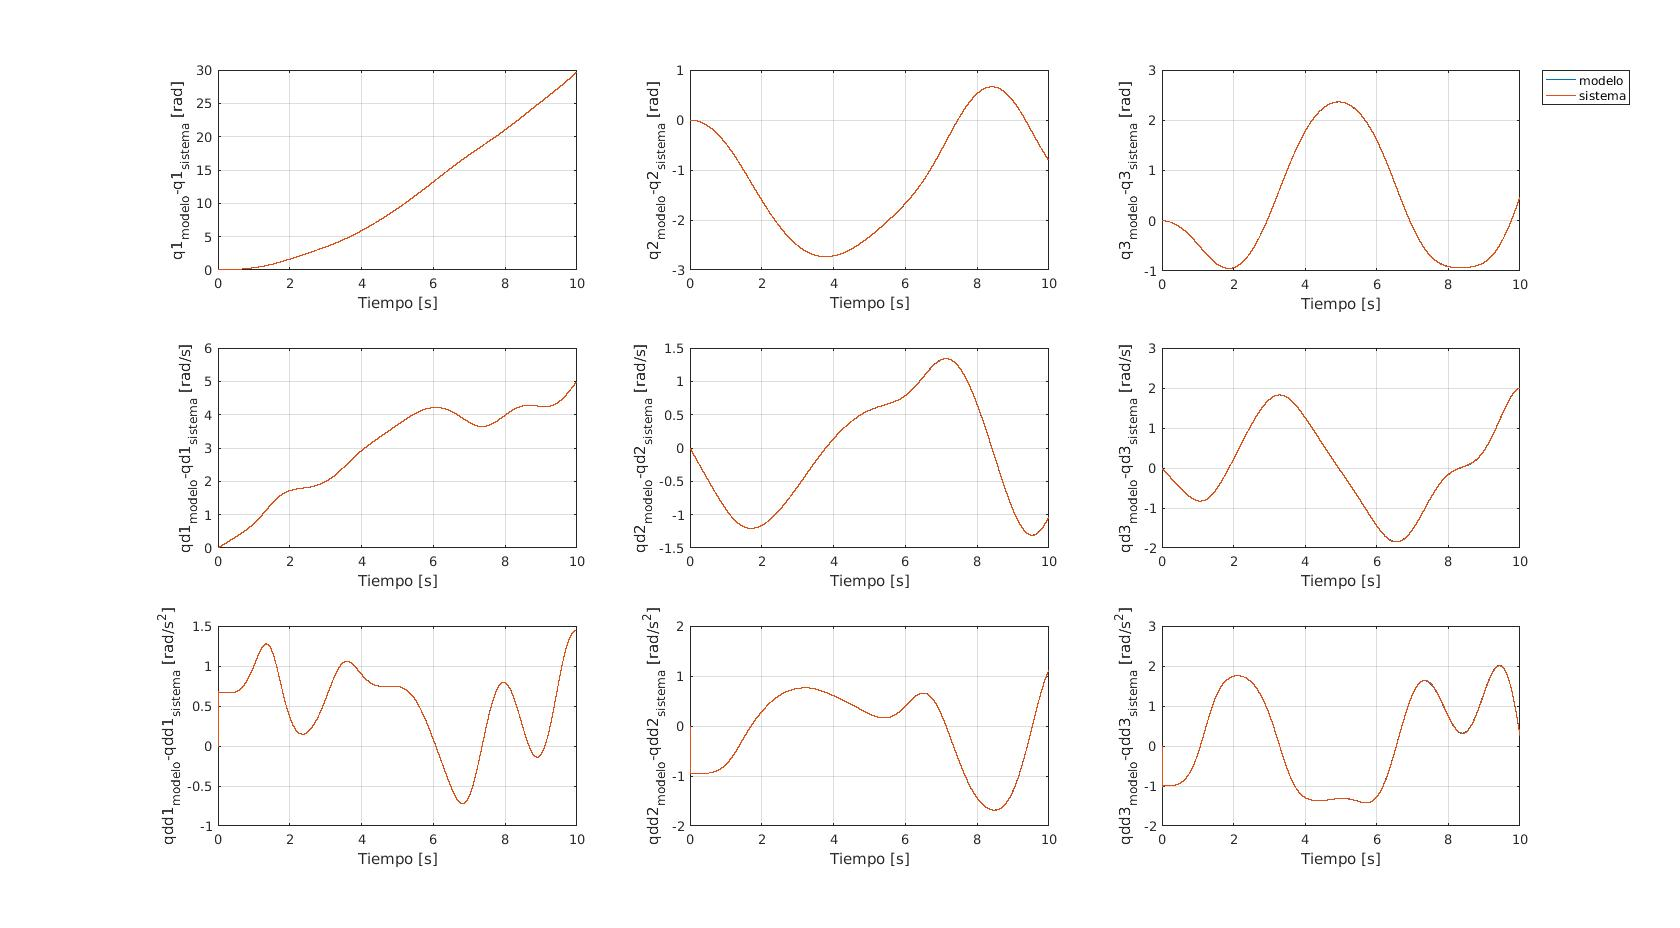
\includegraphics[width=1\textwidth]{EstimacParam_SisMod_In1_IdealCR}
	\caption{Comparativa Variables articulares del modelo obtenido con medidas ideales y reductoras}
\end{figure}

Cómo se puede observar, la magnitud del error será muy baja, por tanto, eso conllevará que se han estimado los parámetros dinámicos del robot con un bajo error entre los parámetros reales.\\
\newpage
A continuación, se mostrará la gráfica del error en las variables articulares:

\begin{figure}[h!]
	\centering
	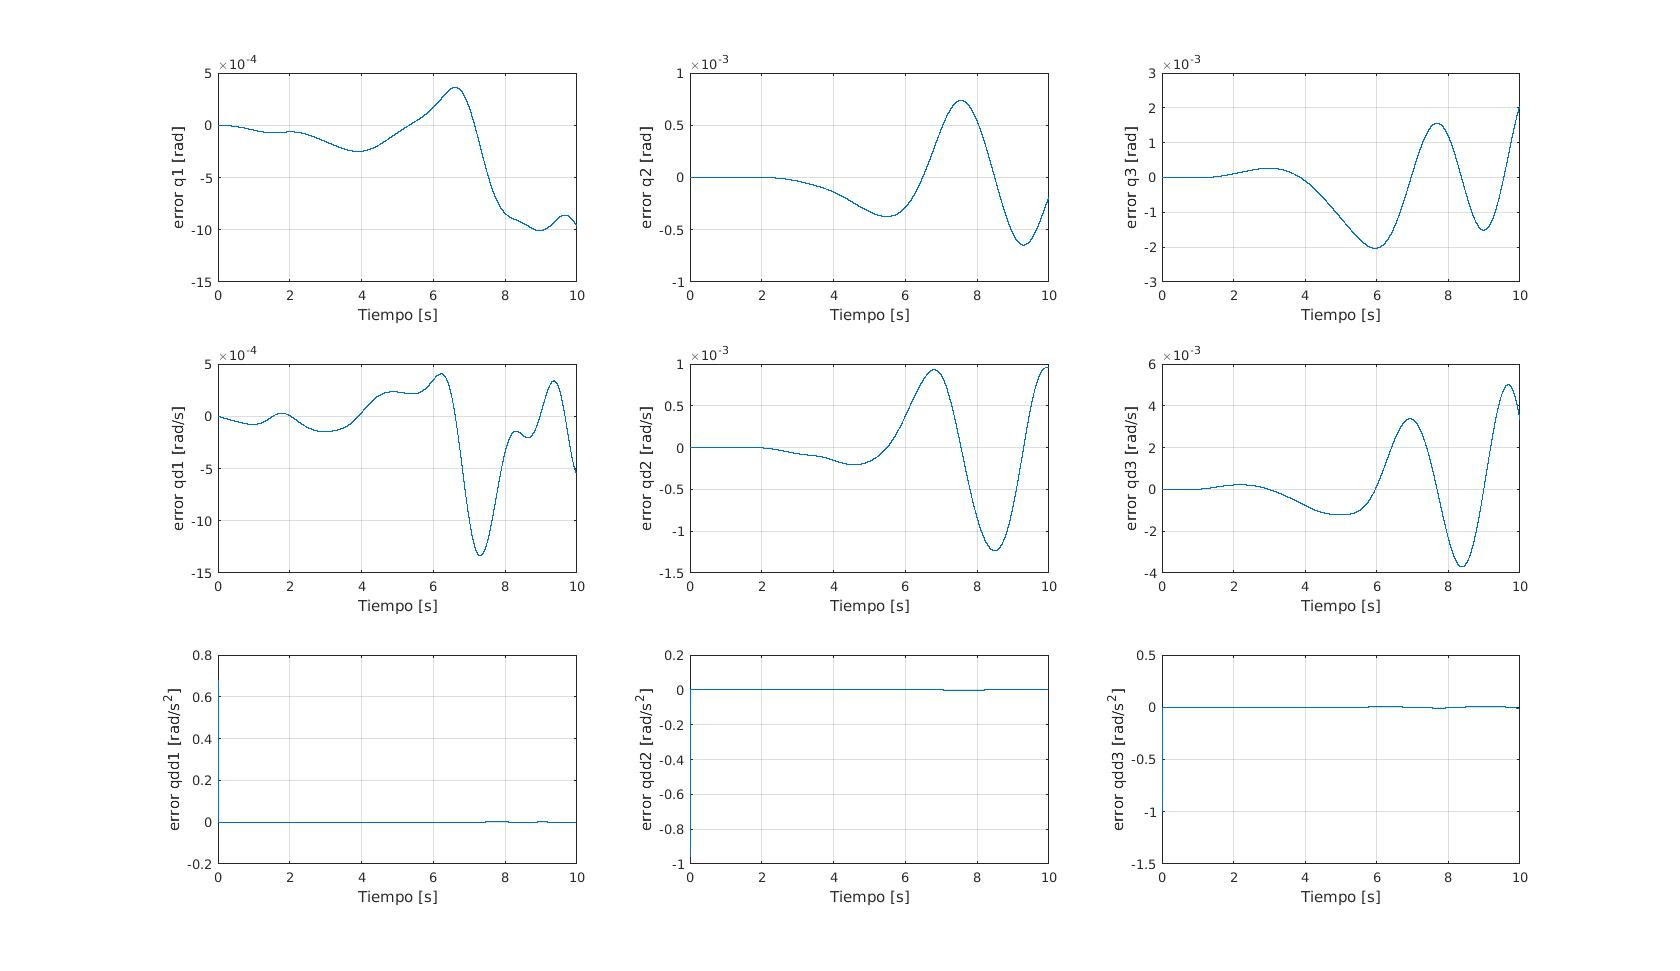
\includegraphics[width=1\textwidth]{EstimacParam_SisModError_In1_IdealCR}
	\caption{Error del modelo obtenido con medidas ideales y reductoras}
\end{figure}

\subsubsection{Robot medidas ideales sin reductoras}
En éste caso, se realizará la misma comparativa que en el caso anterior, con la salvedad es que en el modelo obtenido ahora, se suponen que no se tienen reductoras.\\
Cabe destacar que nos interesa el modelo del robot a bjos tiempos, es decir, los primeros 5 segundos de la simulación, pues no se va a querer controlar el robot en trayectorias que duren más tiempo. Se ha graficado más tiempo para que se observe que, cuando empieza a pasar más del tiempo que se desea controlar, los errores comienzan a incrementarse.\\
A continuación, se mostrará la gráfica resultando al excitar el modelo del sistema y el robot real con intensidades constantes y unitarias.

\newpage
\begin{figure}[h!]
	\centering
	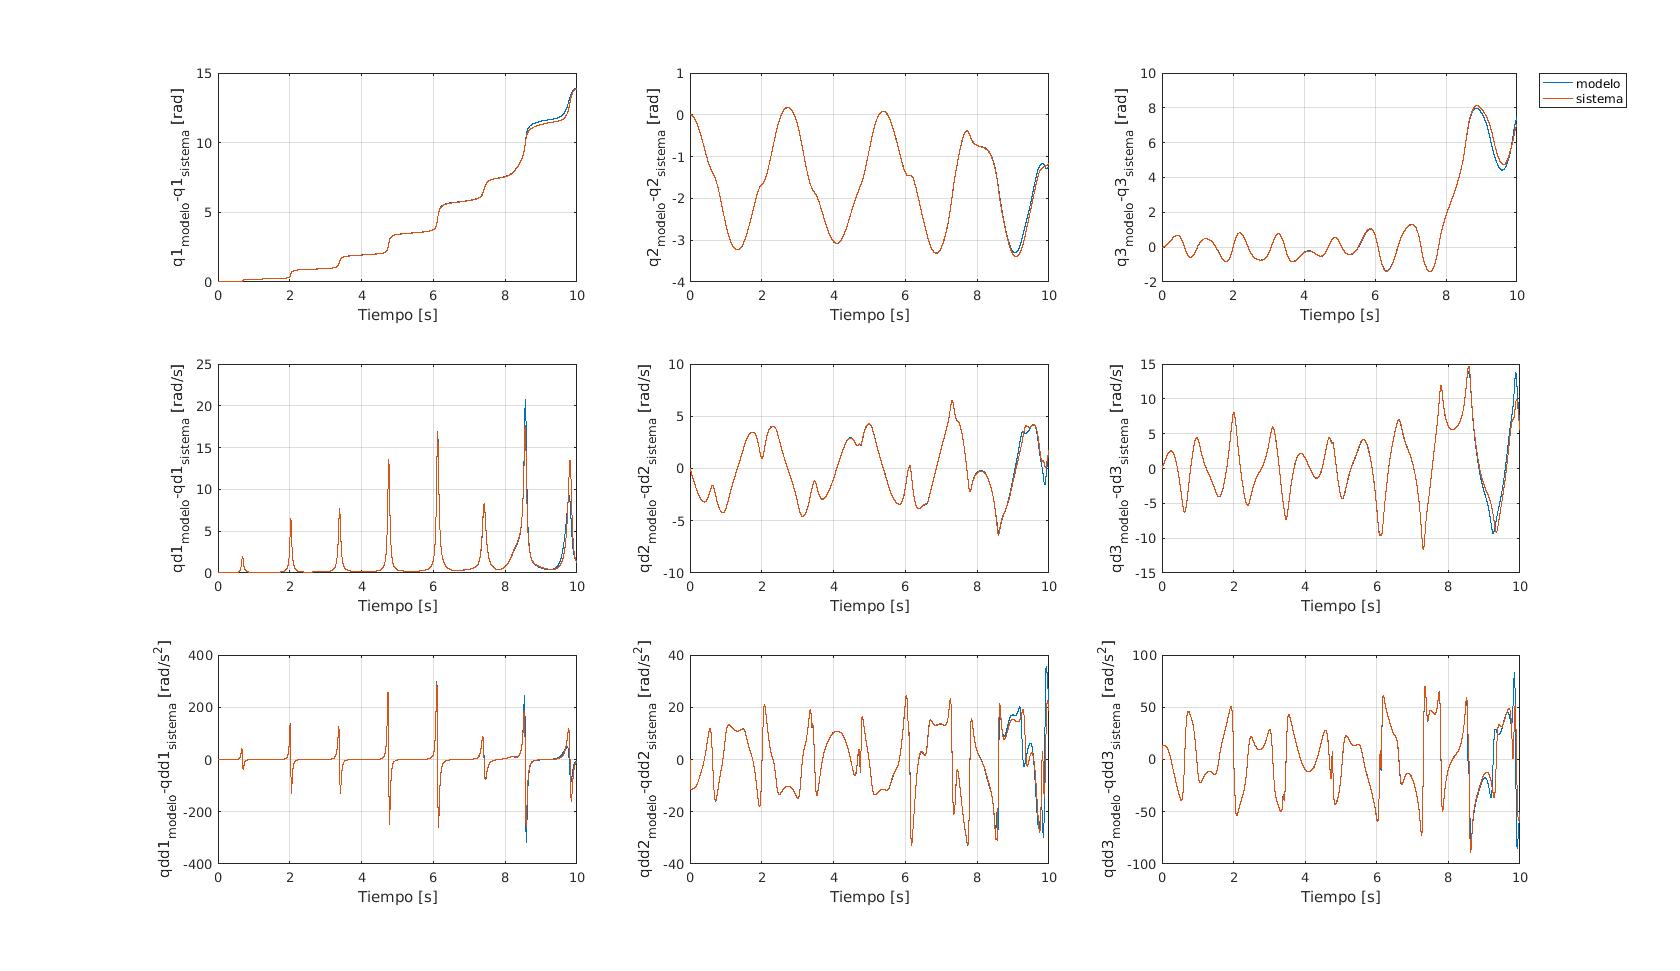
\includegraphics[width=1\textwidth]{EstimacParam_SisMod_In1_IdealSR}
	\caption{Comparativa Variables articulares del modelo obtenido con medidas ideales y sin reductoras}
\end{figure}

Cómo se puede observar, al igual que antes, cuándo se emplean medidas ideales para estimar los parámetros dinámicos del robot y obtener un modelo del mismo, se obtendrán buenos modelos, debido a que cómo se indico antes, las medidas son ideales. \\
Por tanto, a continuación se mostrará la gráfica de los errores de las variables articulares:

\begin{figure}[h!]
	\centering
	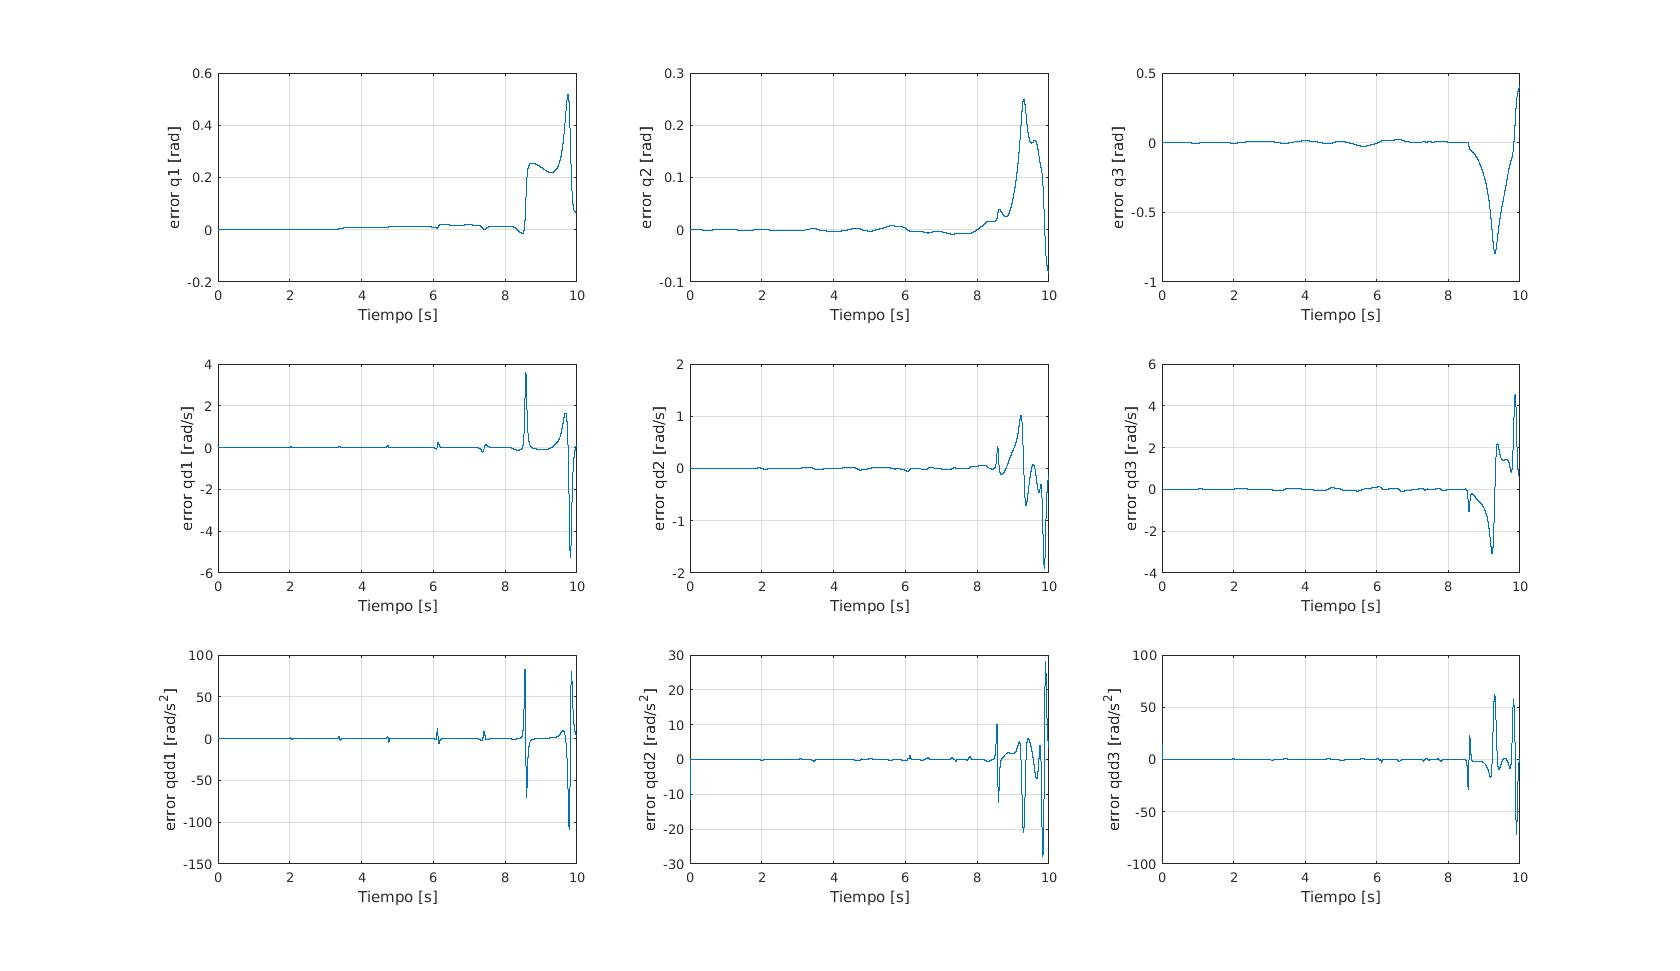
\includegraphics[width=1\textwidth]{EstimacParam_SisModError_In1_IdealSR}
	\caption{Error del modelo obtenido con medidas ideales y sin reductoras}
\end{figure}

\subsubsection{Robot medidas reales con reductoras}
Aunque se haya obtenido el modelo con medidas reales suponiendo que no se tienen tacómetros y que, por tanto, no se puede conocer la velocidad articular del robot, para realizar análisis de control y para análizar el modelo obtenido sí se conocerá la velocidad articular, es decir, se supondrá que se tienen tacómetros. De ese modo se evitará la necesidad de implementar un filtro no causal. \\
Los filtros no causales se caracterizan por el hecho de se emplean valores futuros de la señal, algo que sólo se podrá hacer de manera computacional una vez se hayan tomado todos los datos.\\

Por tanto, se compararán las medidas reales de velocidad y posición del robot con las medidas ideales del modelo obtenido. La grafica comparativa se muestra a continuación:

\begin{figure}[h!]
	\centering
	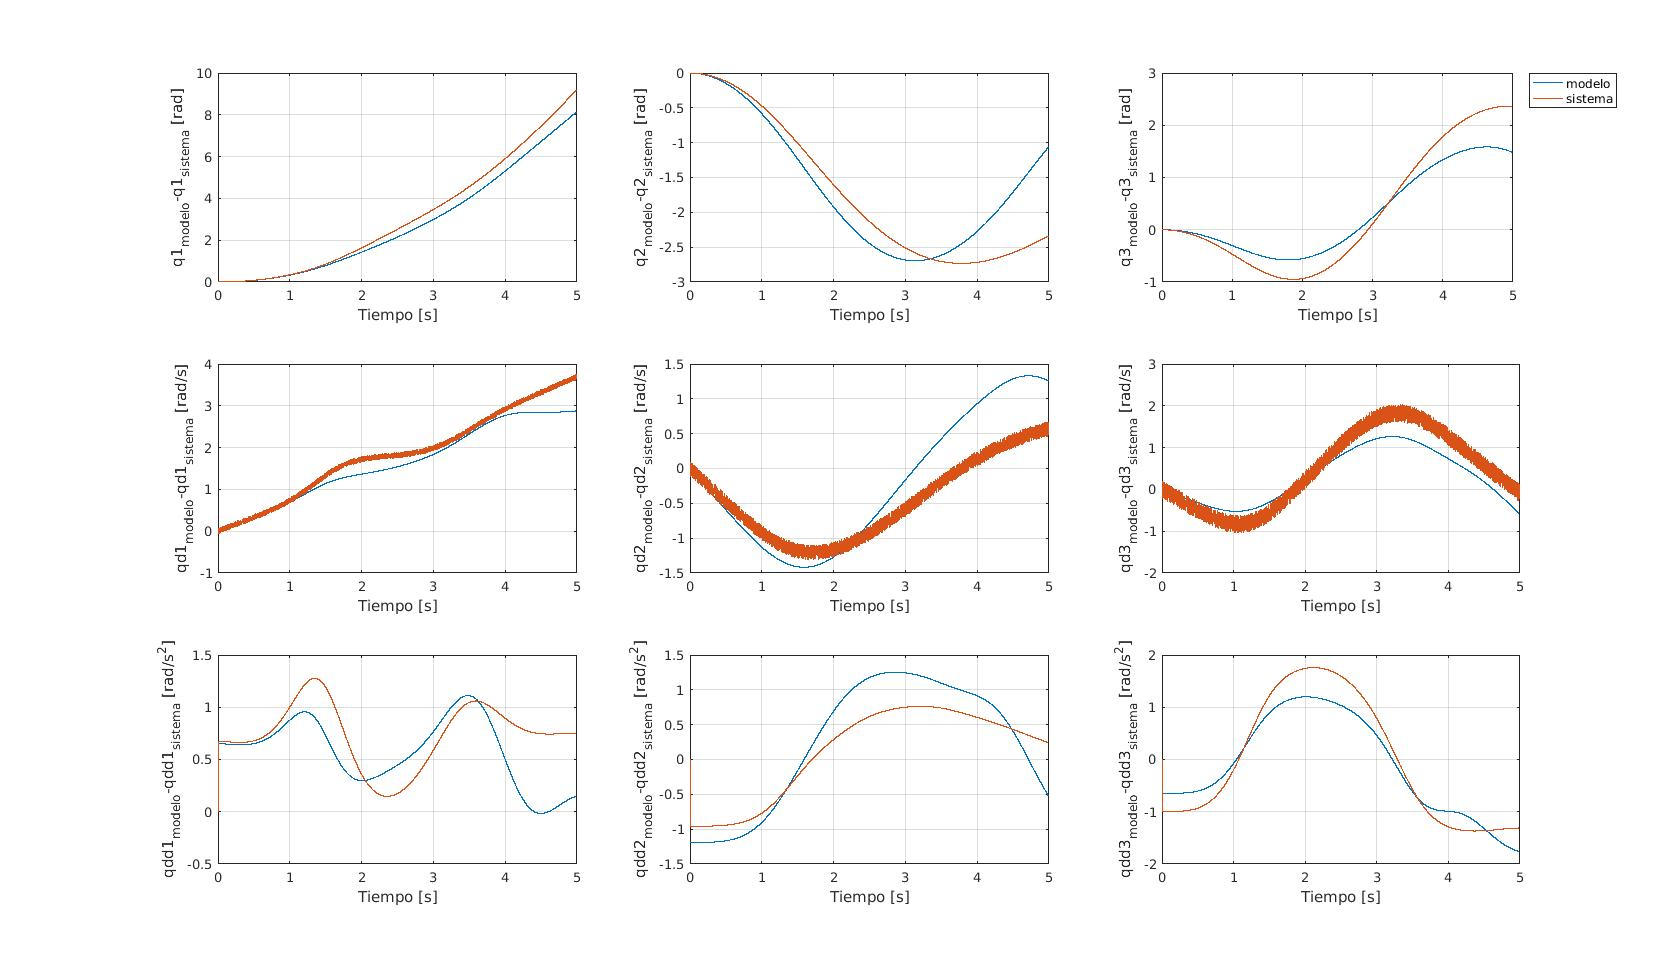
\includegraphics[width=1\textwidth]{EstimacParam_SisMod_In1_RealCR}
	\caption{Comparativa Variables articulares del modelo obtenido con medidas reales y reductoras}
\end{figure}

En éste caso, se observa cómo al emplear medidas reales para obtener el modelo dinámico del robot y al haber tenido que emplear filtros computacionales para conocer velocidades y aceleraciones del robot, el modelo obtenido no será tan bueno cómo en el caso en el que se usaron medidas ideales. Sin embargo, debido a que no posee un elevado orden de magnitud, se asumirá dicho error y se tomará el modelo cómo válido.

\newpage
Por tanto, la magnitud de los errores obtenidos se muestra a continuación:

\begin{figure}[h!]
	\centering
	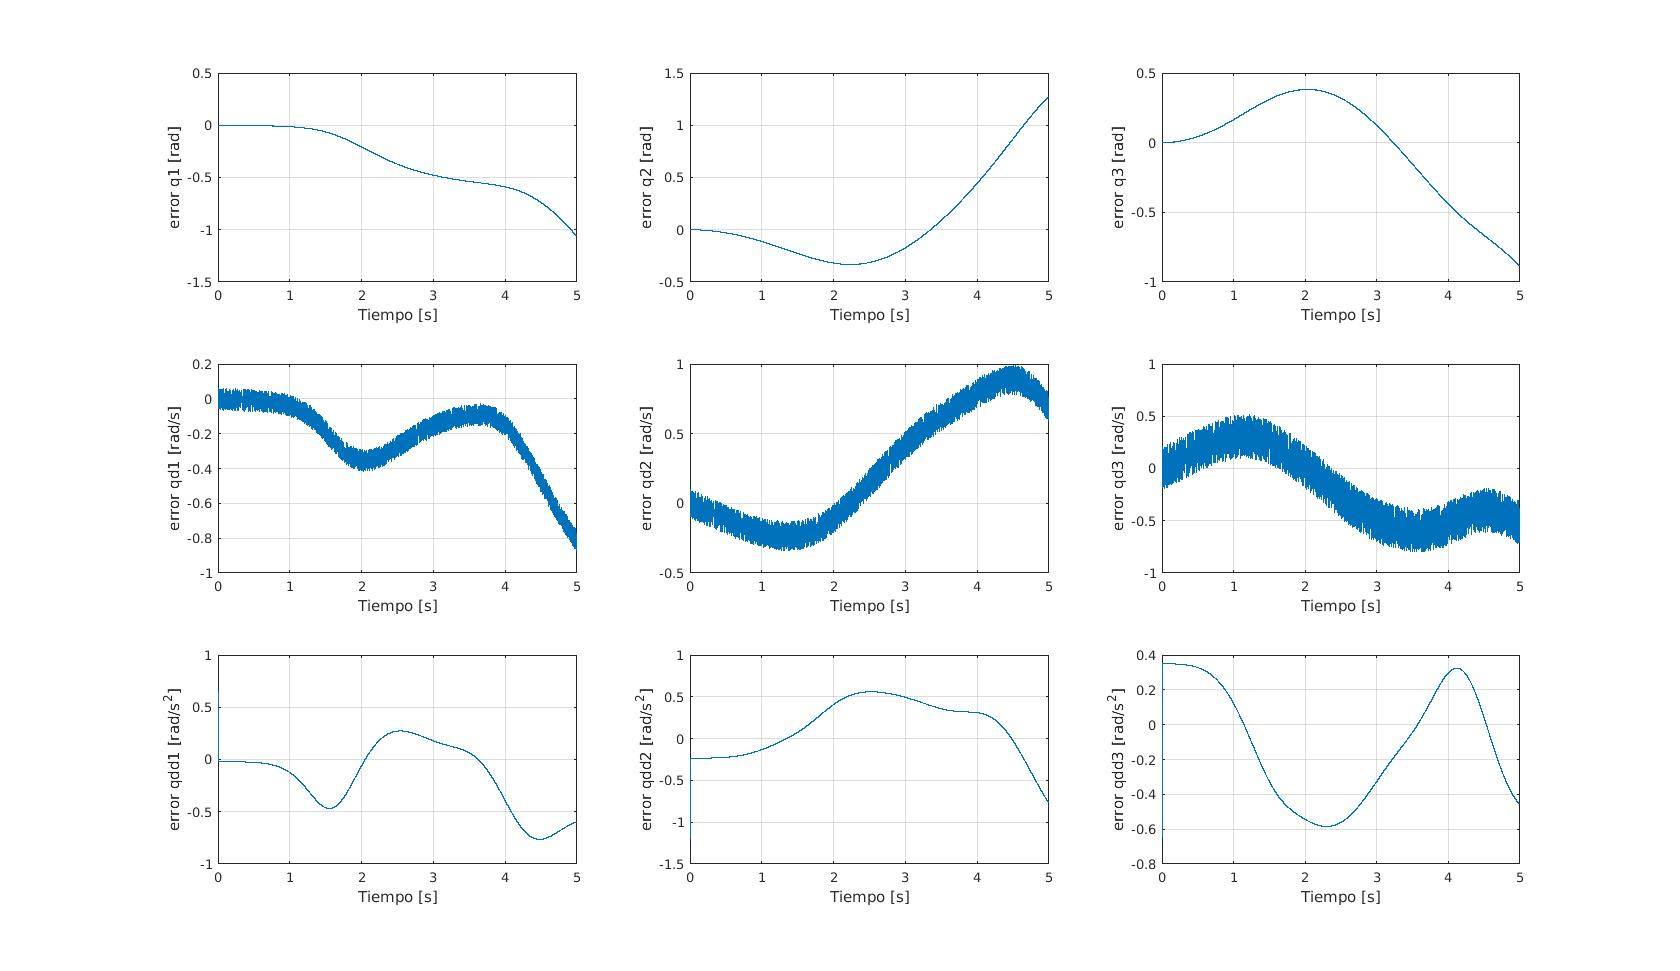
\includegraphics[width=1\textwidth]{EstimacParam_SisModError_In1_RealCR}
	\caption{Error del modelo obtenido con medidas reales y reductoras}
\end{figure}

\subsubsection{Robot medidas reales sin reductoras}
